\epigraph{``\textit{Non-reproducible single occurrences are of no significance to science.}''}{---\citeauthor{popper2005logic}, \citeyear{popper2005logic} \cite{popper2005logic}}

En esta sección de Experimentos, analizaremos y compararemos los tiempos de ejecución y la memoria utilizada por los algoritmos implementados, utilizando gráficos que nos ayuden a visualizar las diferencias significativas entre los enfoques de \textit{Fuerza Bruta} y \textit{Programación Dinámica}. 

\subsubsection{Configuración de los Experimentos}

La recopilación de datos se realiza desde el momento en que se llaman las funciones implementadas en los archivos correspondientes. Estas funciones reciben como parámetros dos cadenas, \( S1 \) y \( S2 \), que representan los datos de entrada. Una vez que la función finaliza su ejecución, se obtienen los siguientes datos de salida:
- La distancia mínima necesaria para transformar \( S1 \) en \( S2 \).
- El tiempo de ejecución medido en segundos y microsegundos.
- La cantidad de memoria gestionada en bytes, recopilada mediante la herramienta \textbf{Valgrind} en el campo \textit{bytes allocated}.

Un ejemplo de ejecución se puede observar en la \cref{fig:ejemplo-ejecución}:

\begin{figure}[H]
    \centering
    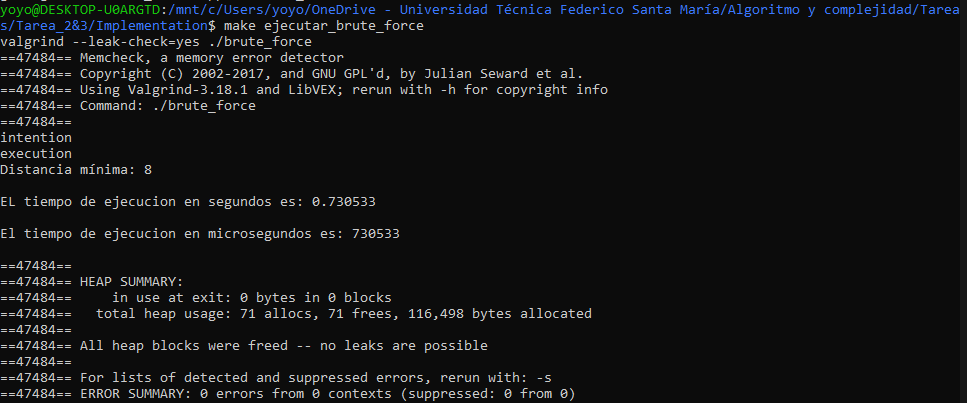
\includegraphics[width=0.75\linewidth]{Tarea_2&3//images/ejemplo_ejecucion.png}
    \caption{Ejemplo de la ejecución del programa con sus respectivas entradas y salidas.}
    \label{fig:ejemplo-ejecución}
\end{figure}

\subsubsection{Entorno de Pruebas}

Para llevar a cabo los experimentos, se utilizó el siguiente hardware y software:

\textbf{Hardware:}
  - Procesador: Intel Core i5-5200U, 2.20 GHz.
  - Memoria RAM: 12 GB.
  - Almacenamiento: Sin SSD.

\textbf{Software:}
  - Sistema Operativo: Windows 10.
  - Terminal: Ubuntu 22.04.3 LTS (en entorno WSL).
  - Compilador: \texttt{g++ 11.4.0}.
  - Librerías utilizadas:
    \texttt{<bits/stdc++.h>}, \texttt{<sys/time.h>}

Esta configuración asegura una ejecución reproducible de los experimentos, permitiendo contrastar los resultados en términos de tiempos de ejecución y uso de memoria bajo condiciones controladas.